% fig05_wakefield_density.tex — Cold-linear wakefield scalings vs plasma
% density: the wave-breaking field E_0 (left axis, GV/m) and the plasma
% wavelength lambda_p (right axis, um) over n_e = 1e16-1e19 cm^-3. The
% 1e18 cm^-3 operating point (the verify-ledger anchor: E_0=96.159 GV/m,
% lambda_p=33.389 um) is marked. Compiled to PDF for Appendix B.
%
% Data: closed forms omega_p=sqrt(n_e e^2/(eps0 m_e)), lambda_p=2 pi c/omega_p,
% E_0=m_e c omega_p/e (Dawson). Reproduces the literature engineering
% coeffs E_0[V/m]~96 sqrt(n_e[cm^-3]) and lambda_p[um]~3.34e10/sqrt(n_e).
% The GV/m gradient (3-4 orders above RF MV/m) is the tabletop motivation.
%
% Manual single-shot compile (debug):
%   xelatex -interaction=nonstopmode -halt-on-error fig05_wakefield_density.tex
\documentclass[border=4pt]{standalone}
\usepackage{tikz}
\usepackage{pgfplots}
\pgfplotsset{compat=1.18}
\begin{document}
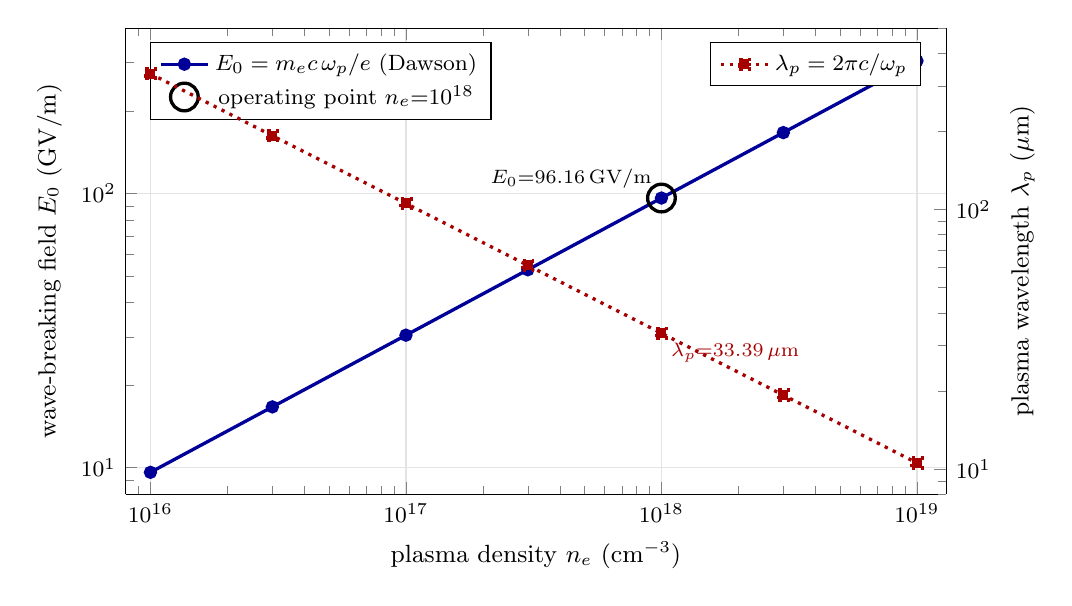
\begin{tikzpicture}
\begin{axis}[
  width=12cm, height=7.5cm,
  xmode=log, ymode=log,
  xlabel={plasma density $n_e$ (cm$^{-3}$)},
  ylabel={wave-breaking field $E_0$ (GV/m)},
  axis y line*=left,
  xmin=8e15, xmax=1.3e19,
  ymin=8, ymax=400,
  tick label style={font=\footnotesize},
  label style={font=\small},
  ymajorgrids, xmajorgrids,
  grid style={gray!22},
  legend pos=north west,
  legend style={font=\footnotesize},
  mark size=1.8pt,
]
\addplot[blue!60!black, very thick, mark=*] coordinates {
  (1e16,9.6159) (3e16,16.6553) (1e17,30.4082) (3e17,52.6686)
  (1e18,96.1592) (3e18,166.5526) (1e19,304.0821)
};
\addlegendentry{$E_0 = m_e c\,\omega_p/e$ (Dawson)}
% mark the 1e18 operating point
\addplot[only marks, mark=o, mark size=5pt, draw=black, very thick] coordinates {
  (1e18,96.1592)
};
\addlegendentry{operating point $n_e{=}10^{18}$}
\node[font=\scriptsize,anchor=south east] at (axis cs:1e18,96.16)
  {$E_0{=}96.16$\,GV/m};
% RF reference band
\addplot[orange!70!black, dashed, thick] coordinates {(8e15,0.05)(1.3e19,0.05)};
\end{axis}
% right axis: plasma wavelength
\begin{axis}[
  width=12cm, height=7.5cm,
  xmode=log, ymode=log,
  axis y line*=right,
  axis x line=none,
  ylabel={plasma wavelength $\lambda_p$ ($\mu$m)},
  xmin=8e15, xmax=1.3e19,
  ymin=8, ymax=500,
  tick label style={font=\footnotesize},
  label style={font=\small},
  legend pos=north east,
  legend style={font=\footnotesize},
  mark size=1.8pt,
]
\addplot[red!65!black, very thick, dotted, mark=square*] coordinates {
  (1e16,333.8943) (3e16,192.7740) (1e17,105.5867) (3e17,60.9605)
  (1e18,33.3894) (3e18,19.2774) (1e19,10.5587)
};
\addlegendentry{$\lambda_p = 2\pi c/\omega_p$}
\node[font=\scriptsize,anchor=north west,text=red!65!black] at (axis cs:1e18,33.39)
  {$\lambda_p{=}33.39\,\mu$m};
\end{axis}
\end{tikzpicture}
\end{document}
